%%%%%%%%%%%%%%%%%%%%%%%%%%%%%%%%%%%%%%%%%%%%%%%%%
% This tex file uses minted package.
% Do not compile if Pygments highlighter for 
% minted is not installed. 
% Use admin to compile this file.
%%%%%%%%%%%%%%%%%%%%%%%%%%%%%%%%%%%%%%%%%%%%%%%%%

\documentclass[12pt,a4paper]{article}
\usepackage{amsmath,amscd,amsbsy,amssymb,latexsym,url,bm,amsthm}
\usepackage{epsfig,graphicx,subfigure}
\usepackage{enumitem,balance}
\usepackage{wrapfig}
\usepackage{mathrsfs,euscript}
\usepackage[usenames]{xcolor}
\usepackage{hyperref}
\usepackage[vlined,ruled,linesnumbered]{algorithm2e}
\hypersetup{colorlinks=true,linkcolor=black}

\newtheorem{theorem}{Theorem}
\newtheorem{lemma}[theorem]{Lemma}
\newtheorem{proposition}[theorem]{Proposition}
\newtheorem{corollary}[theorem]{Corollary}
\newtheorem{exercise}{Exercise}
\newtheorem*{solution}{Solution}
\newtheorem{definition}{Definition}
\theoremstyle{definition}

\renewcommand{\thefootnote}{\fnsymbol{footnote}}

\newcommand{\postscript}[2]
 {\setlength{\epsfxsize}{#2\hsize}
  \centerline{\epsfbox{#1}}}

\renewcommand{\baselinestretch}{1.0}

\setlength{\oddsidemargin}{-0.365in}
\setlength{\evensidemargin}{-0.365in}
\setlength{\topmargin}{-0.3in}
\setlength{\headheight}{0in}
\setlength{\headsep}{0in}
\setlength{\textheight}{10.1in}
\setlength{\textwidth}{7in}
\makeatletter \renewenvironment{proof}[1][Proof] {\par\pushQED{\qed}\normalfont\topsep6\p@\@plus6\p@\relax\trivlist\item[\hskip\labelsep\bfseries#1\@addpunct{.}]\ignorespaces}{\popQED\endtrivlist\@endpefalse} \makeatother
\makeatletter
\renewenvironment{solution}[1][Solution] {\par\pushQED{\qed}\normalfont\topsep6\p@\@plus6\p@\relax\trivlist\item[\hskip\labelsep\bfseries#1\@addpunct{.}]\ignorespaces}{\popQED\endtrivlist\@endpefalse} \makeatother

\usepackage{tikz}
\usepackage{minted}
\renewcommand{\theFancyVerbLine}{\ttfamily
\textcolor[rgb]{0.5,0.5,1.0}{\tiny
\oldstylenums{\arabic{FancyVerbLine}}}}
\setminted{
	breaklines,autogobble,linenos,numbersep=1mm,frame=lines,framesep=2mm,fontsize=\scriptsize,
}
\usepackage{tcolorbox}
\usepackage{array}

\begin{document}
\noindent

%========================================================================
\noindent\framebox[\linewidth]{\shortstack[c]{
\Large{\textbf{Lab03-Greedy Strategy}}\vspace{1mm}\\
CS214-Algorithm and Complexity, Xiaofeng Gao, Spring 2021.}}


\begin{center}
\footnotesize{\color{red}$*$ If there is any problem, please contact TA Haolin Zhou.}\par
% Please write down your name, student id and email.
\footnotesize{\color{blue}$*$ Name: Log Creative \quad Student ID:  \quad Email: logcreative-lzl@sjtu.edu.cn}
\end{center}

\begin{enumerate}
	\item \textit{Interval Scheduling.} Interval Scheduling is a classic problem solved by \textbf{greedy algorithm}: given $n$ jobs and the $j$-th job starts at $s_j$ and finishes at $f_j$. Two jobs are compatible if they do not overlap. The goal is to find maximum subset of mutually compatible jobs. Tim wants to solve it by sort the jobs in descending order of $s_j$. Is this attempt correct? Prove the correctness of such idea, or else provide a counter-example.
	\begin{solution}
		\textbf{Tim is correct.} Prove this idea by contradiction.

		Assume greedy is not optimal for scheduling the jobs in descending order of $s_j$.

		Let $i_1,i_2,\cdots,i_k$ denote set of jobs selected by greedy.

		Let $j_1,j_2,\cdots,j_m$ denote set of jobs in an optimal solution with $i_k=j_m,i_{k-1}=j_{m-1},\cdots,i_{k-r}=j_{m-r}$ for the largest possible value of $r$.

		\begin{figure}[h]
			\centering
			\begin{tikzpicture}
\tikzstyle{timeblock}=[minimum height = 0.6cm,draw=gray!20,fill=gray!20];

\draw (5.5,1.47) -> (-5,1.47);
\draw (5.6,-0.03) -> (-5,-0.03);
\node at (-6,1.5) {Greedy};
\node at (-6,0) {OPT};
\node [timeblock,minimum width=2cm] at (4.4,1.8) {$i_k$};
\node [timeblock,minimum width=2cm] at (4.4,0.3) {$j_m$};
\node [timeblock,minimum width=1.5cm] at (2.5,1.8) {$i_{k-1}$};
\node [timeblock,minimum width=1.5cm] at (2.5,0.3) {$j_{m-1}$};
\node [timeblock,minimum width=1.6cm] at (0,1.8) {$i_{k-r}$};
\node [timeblock,minimum width=1.6cm] at (0,0.3) {$j_{m-r}$};
\draw[dashed] (-0.8,2.6) -- (-0.8,-0.4);
\node [timeblock,minimum width=1.7cm] at (-2,1.8) {$i_{k-(r+1)}$};
\node [timeblock,minimum width=1.6cm,fill=blue!50!black,text=white] at (-2.2,0.3) {$j_{m-(r+1)}$};
\node [timeblock,minimum width=1.6cm,fill=blue!50!black,text=white] at (-4,0.3) {$\cdots$};
\draw[dashed] (-3.05,-0.4) -- (-3.05,2.6);
\draw[->] node [above] at (-2,2.8) {job $i_{k-(r+1)}$ starts after $j_{m-(r+1)}$} edge (-2,2.4);
\draw[->,red] node [below] at (-2.2,-1) {why not replace job $j_{m-(r+1)}$ with job $i_{k-(r+1)}$?} edge (-2.2,-0.2);
\end{tikzpicture}
		\end{figure}

		For job $i_{k-(r+1)}$, it starts after $j_{m-(r+1)}$. But why not replace job $j_{m-(r+1)}$ with job $i_{k-(r+1)}$, so that the solution is still feasible and optimal. Then, it contradicts the maximality of $r$.

		So, the greedy solution is optimal in this case.
	\end{solution}
	
	\item \textit{Done deal.} In a basketball league, teams need to complete player trades through matching contracts. Every player is offered a contract. For the sake of simplicity, we assume that the unit is $ M $, and the size of all contracts are integers. The process of contract matching refers to the equation: $ \sum_{i\in A} a_{i}=\sum_{j\in B} b_{j} $, where $ a_{i} $ refers to the contract value of player $ i $ in team $A$ involved in the trade and $ b_{j} $ refers to the value of player $ j $ in team $B$. 
	
	Assume that you are a manager of a basketball team and you want to get \textbf{one} star player from another team through trade. The contract of the star player is $ n (n\in \mathbb{N}^+) $. The goal is to complete the trade with as few players as possible. 
	
	\begin{enumerate}
		\item Describe a \textbf{greedy} algorithm to get the deal done with the least players in your team. Assume that there are only 4 types of contracts in your team: $25M$, $ 10M $, $ 5M $, $ 1M $, and there is no limit to the number of players. Prove that your algorithm yields an optimal solution.
		\item Suppose that the available contract sizes are powers of $c$,
		i.e., the values are $c^{0}, c^{1}, \ldots, c^{k}$ for some integers $c>1$ and $k \geq 1$. Show that the greedy algorithm always yields an optimal solution.
		\item Give a set of contract sizes for which the greedy algorithm does not yield an optimal solution. Your set should include a $ 1M $ so that there is a solution for every value of $ n $.
	\end{enumerate}
    \begin{solution}
		Explain the greedy algorithm for all three sub-problems. The goal is to find the mimimum size of the collection of contract values such that 
		\begin{equation*}
			\sum_{i\in A} a_i = n
		\end{equation*}

		Firstly, \textbf{to avoid the waste on the expenses} (beacuse there is no limit to the number of players), the summation of values of the trade players should be exactly $n$. Otherwise, just use the biggest type of contract will lead to the optimal solution of one player.

		Then, try to use the maximum value of the type of contract to reduce the remaining value, for each \emph{trading round}. 

		\begin{minipage}{0.94\textwidth}
		\begin{algorithm}[H]
			\KwIn{The contract of the star player $n$, contract type array $\{x_i\}_{x=1}^t$}
			\KwOut{The required amount $N$ of players for the deal}
			\BlankLine
			Sort $\{x_i\}_{i=1}^n$ in a descending order\;
			$N\leftarrow 0$\;
			\For(){$i\leftarrow 1$ to $t$}{
				$N\leftarrow N + \lfloor \frac{n}{x_i}\rfloor$\;
				$n\leftarrow n + (n \mod x_i)$\;
				\lIf{$n=0$}{\textbf{break}}
			}
			\If(){$n>0$}{
				\Return{No greedy solution}\;
			}
			\Return{$N$}\;
			\caption{The greedy algorithm for matching contracts}
		\end{algorithm}
		\end{minipage}
        \begin{enumerate}
		   \item \begin{description}
			   \item[Case 1: Exchange exactly.] If an optimal solution tries to exchange the large size into the small size ones for one trading round, because
			   \begin{align*}
				   25M &= 10M \times 2 + 5M\\
				   10M &= 5M\times 2\\
				   5M &= 1M \times 5
			   \end{align*}
			   yields an optimal solution for the exchange. As is noticed, the required amount of players is bigger than 1. In other word, 2 smaller contracts are least needed to meet the large expense. And the remaining part is structed to use the biggest types of contracts as the greedy algorithm goes, there is no optimization space to reduce the amount of players. So it is not an optimal solution, in order not to waste surplus money.
			   \item[Case 2: Exchange not exactly.] Maybe there may be a not exactly exchange the large size scenario. This will only happen when \textbf{2 sub-size is not enough}, specifically, $25M$ and $5M$. 
			   \begin{description}
				   \item[Case 2a: The least size bigger than $1M$.] For the least size bigger than $1M$, say $5M$, if the part cannot be exchanged by $5M$ (for example, $4M$), then it cannot be done by its multiplier as well.
				   \begin{equation*}
					   x \nmid r \Rightarrow kx \nmid r
				   \end{equation*}
				   where $k\in \mathbb{N}_+, r<x$. Then,
				   \begin{align*}
					   x &\nmid  r + mx\\
					   kx &\nmid r + mx
				   \end{align*}
				   where $m\in\mathbb{N}_+$. So $r$ has to be regarded seperately: $r$ has to be consummed by $1M$.
				   \item[Case 2b: The larger one.] For $25M$, if it is first exchanged by $10M\times 2$, maybe the remaining part is $5M$ additional to $25M$, then one more $10M$ is required. But this takes at least 3 players instead of 2:
				   \begin{equation*}
					   25M + 5M = 10M\times 3
				   \end{equation*}
				   If the remaining part is $6M$ or $4M$, according to Case 2a, you cannot deal with $r=1M$ or $r=4M$ with an optimized allocation, and the bigger part is already allocated by the greedy way:
				   \begin{align*}
					   25M + 5M + 1M &= 10M \times 3 + 1M\\
					   25M + 1M \times 4 &= 10M \times 2 + 5M + 1M \times 4
				   \end{align*}	
			   \end{description}
		   \end{description}
		   
		   So the greedy algorithm is the best solution.

		   \item Notice the neighbored types:
		   \begin{equation*}
			   c^k = c^{k-1}\times c
		   \end{equation*}
		   where $c>1, c\in \mathbb{N}$ and $k\geq 1$.
		   \begin{description}
			   \item[Case 1: $c=2$] Similar to the exactly exchanging scenario, if the optimized method exchange the bigger one with the sub-small one, the amount of required players is definate to be more than the greedy one.
			   \item[Case 2: $c>2$] 
			   \begin{equation*}
				   c^k > c^{k-1} \times 2
			   \end{equation*}
			   In one optimization block, where there is a remainder $r<c$ to be optimized (if $r\geq c$, it should be divided into the smaller-than-$c$ part and bigger part first, because the bigger part is always better to be consummed by the larger type), 
			   \begin{equation*}
				   c^k + r = c^{k-1}\times 2 + c^{k-1}\times (c-2) + r
			   \end{equation*}
			   because $c\nmid r$, $r$ has to be comsummed by $1M$. In fact, this also holds for $c=2$. The greedy solution is the optimal solution.
		   \end{description}
		   \item The collection of unstatisfied sets is $\mathbf{U}=\{S|\exists x_i,x_{i+1}\in S:x_{i+1}<2x_{i}\}$.
		   
		   One example when one type is not two times bigger than the previous type: $1M,7M,10M$, To get $14M$,
		   \begin{equation*}
			   10M + 1M\times 4 = 7M \times 2
		   \end{equation*}
		   The right one is better.
	    \end{enumerate}
    \end{solution}
	
    \item \textit{Set Cover.} \textbf{Set Cover} is a typical kind of problems that can be solved by greedy strategy. One version is that: Given $n$ points on a straight line, denoted as $\{x_i\}_{i=1}^n$, and we intend to use minimum number of closed intervals with fixed length $k$ to cover these $n$ points.
    \begin{enumerate}
    	\item Please design an algorithm based on \textbf{greedy} strategy to solve the above problem, in the form of \emph{pseudo code}. Then please analyze its \emph{worst-case} complexity.
    	\item Please prove the correctness of your algorithm.
    	\item Please complete the provided source code by C/C++ {\color{blue}(The source code \emph{Code-SetCover.cpp} is attached on the course webpage)}, and please write down the output result by testing the following inputs: 
    	\begin{enumerate}
    		\item the number of points $n=7$;
    		\item the coordinates of points
    		$x=\{1,2,3,4,5,6,-2\}$;
    		\item the length of intervals
    		$k=3$.
    	\end{enumerate}
        \textbf{Remark}: Screenshots of running results are also acceptable 
    \end{enumerate}
   \begin{solution}
       \begin{enumerate}
		   \item Each time cover the largest amount of elements at the moment. In order to cover the maximum amount of the elements, the start of the interval is one of the existing element, which is the same as to make the end of the interval to be one of the element. The greedy algorithm is designed as follows:
		   
		   \begin{minipage}{0.88\textwidth}
			\begin{algorithm}[H]
				\KwIn{An array $\{x_i\}_{i=1}^n$ of size $n$, the length of intervals $k=3$}
				\KwOut{The minimum number of closed intervals of length $k$ to cover the array points}
				\BlankLine
				Sort the array $\{x_i\}_{i=1}^n$\;
				$N \leftarrow 0$\;
				\While(){$n>0$}{
					$maxCov\leftarrow 0$\; $maxLabel\leftarrow 0$\;
					\For(){$i \leftarrow 1$ to $n$}{
						$cov\leftarrow 1$\;
						\For(){$j \leftarrow i+1$ to $n$}{
							\lIf(){$x[j]>x[i]+k$}{\textbf{break}}
							$cov\leftarrow cov + 1$\;
						}
						\If{$cov \geq maxCov$}{
							$maxCov\leftarrow cov$\;
							$maxLabel \leftarrow i$\;
						}
					}
					\For(){$j \leftarrow maxLabel + maxCov$ to $n$}{
						$x[j-maxCov]\leftarrow x[j]$\;
					}
					$n\leftarrow n - maxCov$\;
					$N\leftarrow N + 1$\;
				}
				\Return{N}\;
				\caption{Greedy Set Cover Algorithm}
		   \end{algorithm}
		   \end{minipage}
		   
		   To reduce the time complexity on moving elements, the right most end of interval with the same cover number is selected on each loop.

		   The worst case comes from every range could only cover one elements at a time. Then the time complexity comes to:
		   \begin{equation*}
			   T(n) = O(n\log n) + \sum_{i=1}^n 6i = O(n\log n) + 3n(n+1) = O(n^2)
		   \end{equation*}
		   where one next element is scanned for each investigating element, and only one element is removed from the set for each loop.

		   Or there is an another \emph{sub-worst case}. The first element cover will contain all the elements in the set, but the scanning process has to go through every element. The time complexity follows:
		   \begin{equation*}
			   T(n) = O(n\log n) + \sum_{i=1}^n i = O(n^2)
		   \end{equation*}
		   which is the same level of quantity on the time complexity.

		   \item \begin{proof}  
		   \textbf{Proof by contradiction.} 
		   \begin{lemma}[Start from an element]\label{lem:se}
			   It is optimal to select the intervals that start from an element.
		   \end{lemma}
		   \textbf{Proof of Lemma \ref{lem:se}.}

		   \begin{tabular}{m{2cm}|m{7.5cm}|m{5cm}}
			\bfseries Scenario &\bfseries Visual & \bfseries Explaination \\
			\hline
			middle & \begin{tikzpicture}
\tikzstyle{blackdot} = [circle,fill=black,scale=0.5];
\draw (-3.5,0) -- (4,0);
\draw[fill=red,draw=red,fill opacity=0.1]  (0,0) ellipse (1.5 and 1.5);
\node [blackdot,red] at (-1.5,0) {};

\node [blackdot] at (-0.5,0) {};
\node [blackdot] at (1,0) {};
\node [blackdot] at (1.5,0) {};
\node [blackdot] at (2,0) {};
\node [blackdot] at (-2.5,0) {};

\end{tikzpicture}
 & Interval starts from an element.\\
			\hline
			right shift & \begin{tikzpicture}
\tikzstyle{blackdot} = [circle,fill=black,scale=0.5];
\draw (-3.5,0) -- (4,0);
\draw[fill=green,draw=green,fill opacity=0.1]  (0.5,0) ellipse (1.5 and 1.5);
\draw[fill=red,draw=red,fill opacity=0.1]  (1,0) ellipse (1.5 and 1.5);
\node [blackdot,red] at (-1.5,0) {};

\node [blackdot,blue] at (-0.5,0) {};
\node [blackdot] at (1,0) {};
\node [blackdot] at (1.5,0) {};
\node [blackdot] at (2,0) {};
\node [blackdot] at (-2.5,0) {};

\end{tikzpicture}
 & If the interval right shift a little bit, the amount of covered elements increases, then the increased elements could also be covered by the interval starting from the next element (\textcolor{blue}{blue}).\\
			\hline
			left shift & \begin{tikzpicture}
\tikzstyle{blackdot} = [circle,fill=black,scale=0.5];
\draw (-3.5,0) -- (4,0);
\draw[fill=red,draw=red,fill opacity=0.1]  (0,0) ellipse (1.5 and 1.5);
\draw[fill=green,draw=green,fill opacity=0.1]  (-0.5,0) ellipse (1.5 and 1.5);
\node [blackdot,red] at (-1.5,0) {};

\node [blackdot] at (-0.5,0) {};
\node [blackdot] at (1,0) {};
\node [blackdot] at (1.5,0) {};
\node [blackdot] at (2,0) {};
\node [blackdot] at (-2.5,0) {};

\end{tikzpicture}
 & If the interval left shift a little bit and not touching the previous element, then the amount of covered elements will not exceed the middle scenario, because the lengths of the intervals are the same.
		   \end{tabular}
		   
		   Thus, it is always optimal to select those intervals from an element.\hfil \qed \vspace{\parskip}

		   \begin{lemma}[At most one overlap on one side]\label{lem:ov}
			   The intervals selected by the greedy algorithm could only have at most one overlapped area on each side.
		   \end{lemma}
		   \textbf{Proof of Lemma \ref{lem:ov}.} Prove by contradiction. If the intervals $G_k,G_m,G_n$ are selected by the greedy algorithm in selection order ($k<m<n$) and $G_m, G_n$ overlapped with $G_k$ on the same side, they have to be \textbf{both on the left side}. Because the right end of the $G_k$ are already covered and no starting elements could be selected to form an inteval for overlapping.

		   \begin{figure}[H]
			\centering
			\begin{tikzpicture}
\tikzstyle{blackdot} = [circle,fill=black,scale=0.5];
\draw (-3.5,0) -- (4,0);
\draw[fill=red,draw=red!50,fill opacity=0.05]  (1,0) ellipse (1.5 and 1.5);

\node [blackdot,red!75] at (-1.5,0) {};

\node [blackdot,red!50] at (-0.5,0) {};
\node [blackdot,black!50] at (1,0) {};
\node [blackdot,black!50] at (1.5,0) {};
\node [blackdot,black!50] at (2,0) {};
\node [blackdot,red] at (-2.5,0) {};

\draw[fill=red,draw=red!75,fill opacity=0.1]  (0,0) ellipse (1.5 and 1.5);
\draw[fill=red,draw=red!100,fill opacity=0.15]  (-1,0) ellipse (1.5 and 1.5);
\node[red!50] at (1,2) {$G_k$};
\node[red!75] at (0,2) {$G_m$};
\node[red] at (-1.5,2) {$G_n$};
\end{tikzpicture}
		   \end{figure}

		   However, as is shown in the diagram, If $G_m$ is replaced by $G_n$ at the stage $m$, the interval could \textbf{cover more elements} because the overlapping area \textbf{has already been covered} by $G_k$, which makes no effect on the number of covering elements. Then, this contradicts the definition of the greedy algorithm, so there could only be at most one overlapping area on each side.\hfil \qed \vspace{\parskip}

		   Then, to construct the optimized solution, the overlapping area has to be reduced comparing to the greedy solution. 

		   \begin{figure}[H]
			   \centering
			   \begin{tikzpicture}
\tikzstyle{blackdot} = [circle,fill=black,scale=0.5];
\draw (-3.5,0) -- (4,0);
\draw[fill=red,draw=red!50,fill opacity=0.05]  (1,0) ellipse (1.5 and 1.5);

\node [blackdot,red!75] at (-1.5,0) {};

\node [blackdot,red!50] at (-0.5,0) {};
\node [blackdot,black!50] at (1,0) {};
\node [blackdot,black!50] at (1.5,0) {};
\node [blackdot,black!50] at (2,0) {};
\node [blackdot] at (-2.5,0) {};

\draw[fill=red,draw=red!75,fill opacity=0.1]  (0,0) ellipse (1.5 and 1.5);
\draw[fill=green,draw=green,fill opacity=0.15]  (-2,0) ellipse (1.5 and 1.5);
\node[red!50] at (1,2) {$G_k$};
\node[red!75] at (0,2) {$G_m$};
\node[green] at (-2,2) {$O_m$};
\node at (-0.5,-0.5) {$x_k$};
\end{tikzpicture}
		   \end{figure}

		   Now, consider the overlapped two greedy intervals $G_k,G_m(k<m)$. To reduce the overlapping, construct the optimized interval $O_m$ end at $x_k$ where $G_k$ started and replace $G_m$ by $O_m$. However, $O_m$ will cover more elements than $G_m$ as left shift of the interval will introduce more covered elements and the right overlapping side is the same for no improvement, \textbf{which conflicts the choice of greedy algorithm} at the stage $m$. So no overlapping could be improved and a better optimized interval does not exist. The greedy solution is the optimal solution. 
		\end{proof}
		% Probably consider the triangle inequality?

		%    \item \textbf{Proof by contradiction.} If the cover sets $G_1,G_2,\cdots,G_k$ generated by greedy algorithm, which is ordered in the selected order, is not the optimal, then there exists an optimal solution $O_1,O_2,\cdots,O_l (l<k)$, which is also sorted in the descending order on the size of covers. 
		   
		%    Suppose the two collection differs from the label $i+1$, where $G_1,\cdots, G_i$ and $O_1,\cdots, O_i$ are the same. Investigate the optimal one $O_{i+1}$ and the greedy one $G_{i+1}$.

		%    \begin{description}
		% 	   \item[Case 1: They are of the same size.] Then, there is no contribution in reducing the amount of covers, though it is also a feasible solution, but no fundamentally change. To get a better one, the optimal solution must have a cover set differs from the greedy one in size.
		% 	   \item[Case 2: The optimal one covers more than the greedy one.] Impossible, because the set what greedy algorithm constructs requires to be the best cover at the time.
		% 	   \item[Case 3: The optimal one covers less than the greedy one.] In this case, because the optimal sets have been sorted in the descending order on size, any of the remaining sets could cover strictly less than $\mid G_{i+1} \mid$.
		%    \end{description}
		%    then there exists one of the greedy interval could be shifted in order to cover more elements in the optimal solution. As a result, the number of sets could be reduced in an optimal way.
		   
		% 	Then, there must be an optimal cover set to cover more elements at the time. 

		%    Suppose the collection of cover sets in the greedy solution is denoted as $G_1,\cdots, G_k$, which is labeled in the selected order. 
		%    Because the construction of the greedy algorithm, $G_1,\cdots, G_k$ are not touched, i.e., there is no intersection between any two intervals.
		%    According to the assumption, there exists an element $x$ in $S_i$, such that $x\in S_{i-1}$. 
		   \item 

		   \fbox{\texttt{Code-SetCover.cpp}}

		   \inputminted[]{cpp}{Code-SetCover.cpp}%

		   The output is:
		   \begin{tcolorbox}
			3
		   \end{tcolorbox}
		   
	   \end{enumerate}
   \end{solution}

\end{enumerate}



\vspace{20pt}

\textbf{Remark:} You need to include your .pdf and .tex files in your uploaded .rar or .zip file.

%========================================================================
\end{document}
